% $Id: intro.tex 6021 2007-11-19 15:03:56Z alexandra $
% Local Variables:
% ispell-check-comments: nil
% Local IspellDict: american
% End:
% --------------------------------------------------------
% User documentation
% copyright by BREDEX GmbH 2004
% --------------------------------------------------------
The following sections describe the test hierarchy in \jb{}. 
Basically, you can think of the test hierarchy as a tree structure
which can be of any size, complexity and depth
(\bxfigref{treestructure}).

\begin{figure}
\begin{center}
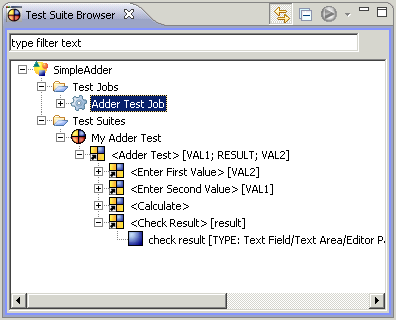
\includegraphics{Concepts/PS/treestructure}
\caption{Test Hierarchy}
\label{treestructure}
\end{center}
\end{figure}

The hierarchical structure of \jb{} gives you flexibility in your
tests to make changes and keep the test in touch with current software
development.

